% Created 2013-02-28 Thu 14:25
\documentclass[11pt]{article}
\usepackage[utf8]{inputenc}
\usepackage[T1]{fontenc}
\usepackage{fixltx2e}
\usepackage{graphicx}
\usepackage{longtable}
\usepackage{float}
\usepackage{wrapfig}
\usepackage{soul}
\usepackage{textcomp}
\usepackage{marvosym}
\usepackage{wasysym}
\usepackage{latexsym}
\usepackage{amssymb}
\usepackage{hyperref}
\tolerance=1000
\DeclareUnicodeCharacter{22EE}{⋮}
\author{G. Jay Kerns}
\date{\today}
\title{Org-mode and julia: an introduction}
\hypersetup{
  pdfkeywords={},
  pdfsubject={},
  pdfcreator={Generated by Org mode 7.9.3e in Emacs 24.3.50.1.}}
\begin{document}

\maketitle
\tableofcontents
\vspace*{1cm}

One of the reasons for this document is that I wanted to make it easier to get acquainted with \texttt{julia}.  

\section{What you need to get started}
\label{sec-1}

This document assumes you have at least a passing familiarity with Org-mode and Emacs keybindings.  

\begin{verbatim}
(load "/path/to/ob-julia.el")
(org-babel-julia-initiate-session "*julia*" nil)
\end{verbatim}

\begin{description}
\item[Note:] a lot of the code blocks below have the header argument \texttt{:eval no-export} which means that the code block can be evaluated interactively in this session by \texttt{C-c C-c} with point in the code block but will \emph{not} be evaluated during export.  The reason is that those blocks have settings which conflict with my current setup but would be useful for others going through this document.
\end{description}

\subsection{Julia}
\label{sec-1-1}
\begin{itemize}
\item First install takes the longest, later updates not so bad.
\item all the dependencies
\end{itemize}
\subsection{Add-on packages}
\label{sec-1-2}

Based on \href{http://www.johnmyleswhite.com/notebook/2012/12/02/the-state-of-statistics-in-julia/}{The State of Statistics in Julia} by John Myles White.

\begin{verbatim}
Pkg.add("DataFrames", "Distributions", "GLM", "MCMC", "Optim", 
        "NHST", "Clustering")
\end{verbatim}

\begin{verbatim}
Pkg.add("RDatasets")
\end{verbatim}


\begin{enumerate}
\item Winston
\label{sec-1-2-1}

The most stable and fully featured of the \texttt{julia} graphics packages at the time of this writing appears to be the \texttt{Winston} package, among alternatives including \texttt{Gadfly}.

\begin{verbatim}
Pkg.add("Winston")
\end{verbatim}

The Winston package has lots of dependencies and many of them must be built from source (on Ubuntu).
\item Gadfly
\label{sec-1-2-2}

\begin{verbatim}
Pkg.add("Gadfly")
\end{verbatim}

\begin{itemize}
\item packages take a lot longer to load than R
\end{itemize}
\end{enumerate}
\subsection{Org-mode}
\label{sec-1-3}

This document assumes that you have at least a passing familiarity with org-mode such that you likely have something like the following already in your \texttt{.emacs}:

\begin{verbatim}
(require 'org)
\end{verbatim}

Another handy setting to have is

\begin{verbatim}
(setq org-confirm-babel-evaluate nil)
\end{verbatim}

In order to run this org file you will need to load \texttt{ob-julia.el} at some point. One way is to edit the following code block and then \texttt{C-c C-c} with point inside the block:

\begin{verbatim}
(load "/path/to/ob-julia.el")
(org-babel-julia-initiate-session "*julia*" nil)
\end{verbatim}

The first command loads the \texttt{ob-julia.el} file and the second initiates a \texttt{julia} session in a buffer called \texttt{*julia*}.  An alternative method is to put the following in your \texttt{.emacs} (these should go below the \texttt{(require 'org)} line):

\begin{verbatim}
(add-to-list 'load-path "/path/to/ob-julia.el")
(org-babel-do-load-languages
 'org-babel-load-languages
 '((emacs-lisp . t)
   (julia . t)))
\end{verbatim}

The following lines (either here or in your \texttt{.emacs}) allow for inline image display in the Emacs buffer.

\begin{verbatim}
(add-hook 'org-babel-after-execute-hook 'org-display-inline-images)   
(add-hook 'org-mode-hook 'org-display-inline-images)
\end{verbatim}

If you'd like to do \LaTeX{} export then put the following in your emacs.

\begin{verbatim}
(require 'ox-latex)
(require 'ox-beamer)
\end{verbatim}
\subsection{ESS - Emacs Speaks Statistics}
\label{sec-1-4}

The place to get the latest version of ESS is \href{http://stat.ethz.ch/ESS/index.php?Section=download}{here}.  

\begin{verbatim}
(add-to-list 'load-path "/path/to/ESS/lisp")
(require 'ess-site)
\end{verbatim}

\begin{verbatim}
(setq  inferior-julia-program-name "/path/to/julia-release-basic")
\end{verbatim}

\section{Prerequisites}
\label{sec-2}

\subsection{Org-mode}
\label{sec-2-1}

\subsection{ESS}
\label{sec-2-2}

\subsection{julia}
\label{sec-2-3}
\section{Interactive session evaluation}
\label{sec-3}

This is about ESS.
\section{Evaluation inside the Org buffer}
\label{sec-4}

\subsection{:results value}
\label{sec-4-1}

\subsection{:results output}
\label{sec-4-2}
\section{Graphics}
\label{sec-5}

The most stable and fully featured of the \texttt{julia} graphics packages at the time of this writing appears to be the \texttt{Winston} package, among alternatives including \texttt{Gadfly}.

\begin{verbatim}
Pkg.add("Winston")
\end{verbatim}

The Winston package has lots of dependencies and many of them must be built from source (on Ubuntu).


\subsection{Plotting with Winston}
\label{sec-5-1}

\begin{verbatim}
using Winston
x = linspace(0, 3pi, 100)
c = cos(x)
s = sin(x)
p = FramedPlot();
setattr(p, "title", "title!")
setattr(p, "xlabel", L"\Sigma x^2_i")
setattr(p, "ylabel", L"\Theta_i")
add(p, FillBetween(x, c, x, s) )
add(p, Curve(x, c, "color", "red") )
add(p, Curve(x, s, "color", "blue") )
file(p, "example1.png")
\end{verbatim}

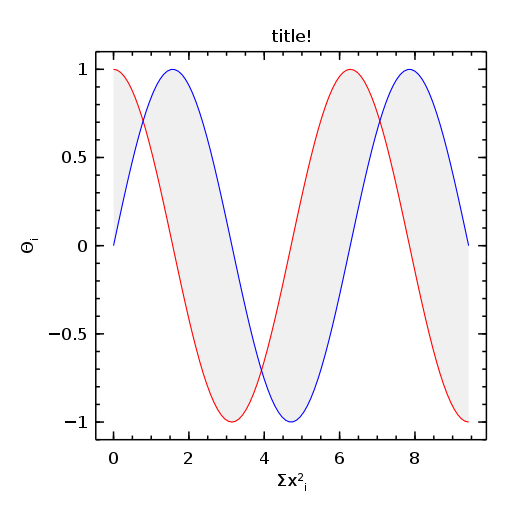
\includegraphics[width=.9\linewidth]{example1.png}

\subsection{Plotting with Gadfly}
\label{sec-5-2}

\begin{verbatim}
using RDatasets
using Gadfly
using Compose
iris = data("datasets", "iris")
p = plot(iris, {:x => "Sepal.Length", :y => "Sepal.Width"}, Geom.point);
SVG("iris_plot.svg", 6inch, 4inch)
\end{verbatim}
\section{Exporting to other formats}
\label{sec-6}

\subsection{\LaTeX{}}
\label{sec-6-1}

\subsection{HTML}
\label{sec-6-2}

\subsection{Beamer}
\label{sec-6-3}
\section{Other things}
\label{sec-7}

\begin{itemize}
\item empty lines in output for semicoloned lines
\item need to start session first
\item when :results value be careful because of readcsv
\begin{itemize}
\item characters
\item 1x1 matrix
\end{itemize}
\end{itemize}
\section{Fitting (generalized) linear models}
\label{sec-8}

\begin{verbatim}
using RDatasets, DataFrames, Distributions, GLM
trees = data("datasets", "trees");
treeslm = lm(:(Girth ~ Height + Volume), trees);
coef(treeslm)
coeftable(treeslm)
\end{verbatim}

\begin{verbatim}
Warning: New definition show(Any,LmMod) is ambiguous with show(IO,ANY) at show.jl:6.
         Make sure show(IO,LmMod) is defined first.
Warning: New definition show(Any,GlmMod) is ambiguous with show(IO,ANY) at show.jl:6.
         Make sure show(IO,GlmMod) is defined first.
WARNING: strcat is deprecated, use string instead.
WARNING: qrd is deprecated, use qrfact instead.
3-element Float64 Array:
 10.8164   
 -0.0454835
  0.19518
3x4 DataFrame:
          Estimate Std.Error  t value   Pr(>|t|)
[1,]       10.8164    1.9732  5.48165 7.44691e-6
[2,]    -0.0454835 0.0282621 -1.60935   0.118759
[3,]       0.19518 0.0109553  17.8161 8.2233e-17
\end{verbatim}
% Generated by Org mode 7.9.3e in Emacs 24.3.50.1.
\end{document}